\section{The SIR Model}
To explain the concepts of ABS and of our functional reactive approach to it, we introduce the SIR model as a motivating example. The SIR model is a a very well studied and understood compartment model from epidemiology which allows to simulate the dynamics of an infectious disease spreading through a population. In this model, people in a population of size $N$ can be in either one of three states \textit{Susceptible}, \textit{Infected} or \textit{Recovered} at a particular time, where it is assumed that initially there is at least one infected person in the population. People interact with each other \textit{on average} with a given rate $\beta$ per time-unit and get infected with a given probability $\gamma$ when interacting with an infected person. When infected, a person recovers \textit{on average} after $\delta$ time-units and is then immune to further infections. An infected person interaction with another infected one is never re-infected, thus interactions amongst infected people is not important in this model. This definition gives rise to three compartments with the transitions as seen in Figure \ref{fig:sir_transitions}.

\begin{figure}
	\centering
	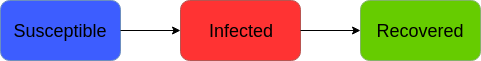
\includegraphics[width=.4\textwidth, angle=0]{./fig/SIR_transitions.png}
	\caption{Transitions in the SIR compartment model.}
	\label{fig:sir_transitions}
\end{figure}

The dynamics of this model over time can be formalized using the following equations:

$\frac{\mathrm d S}{\mathrm d t} = -infectionRate$ \\
$\frac{\mathrm d I}{\mathrm d t} = infectionRate - recoveryRate$ \\
$\frac{\mathrm d R}{\mathrm d t} = recoveryRate$ \\

$infectionRate = \frac{I \beta S \gamma}{N}$ \\
$recoveryRate = \frac{I}{\delta}$ \\

Solving these can be done using the System-Dynamics (SD) approach which solves the equations by integrating over time. In the SD terminology, the intergrals are called \textit{Stocks} and the values over which is integrated over time are called \textit{Flows} \footnote{The $+1$ in $I(t)$ amounts to the initially infected agent - if there wouldn't be a single infected one, the system would immediately reach equilibrium.}.

$S(t) = N + \int_0^t -infectionRate\, \mathrm{d}t$ \\
$I(t) = 1 + \int_0^t infectionRate - recoveryRate\, \mathrm{d}t$ \\
$R(t) = \int_0^t recoveryRate\, \mathrm{d}t$ \\

There exist a huge number of software-packages which allow to conveniently express SD models using a visual approach like in Figure \ref{fig:sir_sd_stockflow_diagramm}.

\begin{figure}
	\centering
	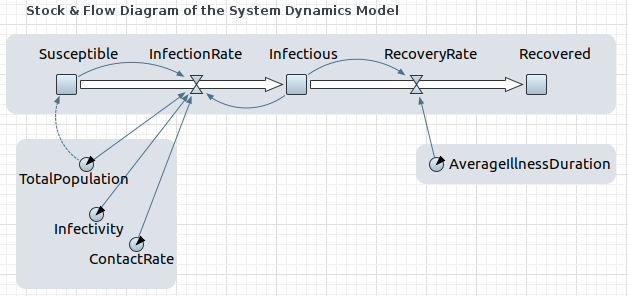
\includegraphics[width=.4\textwidth, angle=0]{./fig/SIR_SD_STOCKFLOW_DIAGRAMM.png}
	\caption{A visual representation of the stocks and flows of the SIR compartment model in the AnyLogic Software.}
	\label{fig:sir_sd_stockflow_diagramm}
\end{figure}

Running the SD simulation over time results in the dynamics as shown in Figure \ref{fig:sir_sd_dynamics_anylogic} with the given variables.

\begin{figure}
	\centering
	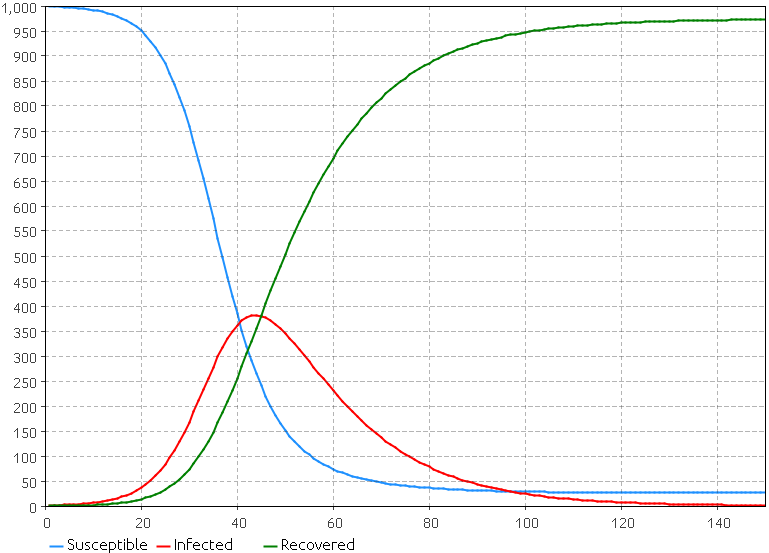
\includegraphics[width=.4\textwidth, angle=0]{./fig/SIR_SD_DYNAMICS_ANYLOGIC.png}
	\caption{Dynamics of the SIR compartment model using the System Dynamics approach. Population Size $N$ = 1000, contact rate $\beta = 1/5$, infection probability $\gamma = 0.05$, illness duration $\delta = 15$. 1 initially infected agent. Simulation run of 150 time-steps. Dynamics generated with AnyLogic Personal Learning Edition 8.1.0.}
	\label{fig:sir_sd_dynamics_anylogic}
\end{figure}

\subsection{An Agent-Based approach}
The SD approach is inherently Top-Down because the emergent property of the system is formalized in differential equations. The question is if such a top-down behaviour can be emulated using ABS, which is inherently bottom-up. Also the question is if there are fundamental drawbacks and benefits when doing so using ABS. Indeed such questions were asked before and modelling the SD approach of the SIR model is possible using an agent-based approach. It is important to note that SD treats the population completely continuous which results in non-discrete values of stocks e.g. 3.1415 infected persons. Thus the fundamental approach to map the SIR model to an ABS is to discretisize the population and model each person in the population as an invidivual agent. The transition  between the states are no longer happening according to continuous differential equations but due to discrete events caused both by interactions amongst the agents and time-outs. The behaviour can be defined as follows:

\begin{itemize}
	\item Every agent makes on average contact with $\beta$ random other agents per time unit. In ABS we can only contact discrete agents thus we model this by generating a random event on average every $\beta$ time units (Note that this ammounts to sampling from an exponential CDF).
	
	\item An agent does not know the other agents' state when making contact with it, thus we need a mechanism in which agents reveal their state in which they are in \textit{at the moment of making contact}. Obviously the already mentioned messaging-mechanism which allows agents to interact is perfectly suited to do this.
	\begin{itemize}
		\item \textit{Susceptible} agent: sends a "Susceptible" message when contacting another agent. There is no need to reply to other incoming messages as making contact with a susceptible agent has no influence on the state of an agent.
		\item \textit{Infected} agent: An infected agent needs to reply to incoming "Susceptible" messages with an "Infected" message to let the susceptible agent know that it has made contact with an infected agent. Note that an infected agent must not sends a "Infected" message by initiated on its own as this would lead to false results (TODO: better argumentation).
		\item \textit{Recovered} agent: does not need to send messages because contacting it or being contacted by it has no influence on the state.
	\end{itemize}
	
	\item Susceptible to Infected: needs to have made contact with an infected agent which happens when it receives an "Infected" message. If this occurs an infection occurs with a probability of $\gamma$. The infection can be calculated by drawing from a uniform random-distribution between 0 and 1 and comparing the value to $\gamma$, if the drawn value $p < \gamma$ then infection occurs. Note that this needs to be done for \textit{every} received "Infected" message.
	
	\item Infected to Recovered: a person recovers \textit{on average} after $\delta$ time unites. This is implemented by drawing the duration from an exponential distribution (TODO: borchschev) with $\lambda = \frac{1}{\delta}$ and making the transition after this duration.
\end{itemize}

We will discuss the implementation of this approach in the following sections and as will be shown FrABS will allow us to express this behaviour very explicitly looking very much like a formal ABS specification of the problem. In Figure \ref{fig:sir_abs_anylogic_agents} we give the dynamics simulating the SIR model with the agent-based approach. 
\begin{figure*}
\begin{center}

	\begin{tabular}{c c c}
		\begin{subfigure}[b]{0.3\textwidth}
			\centering
			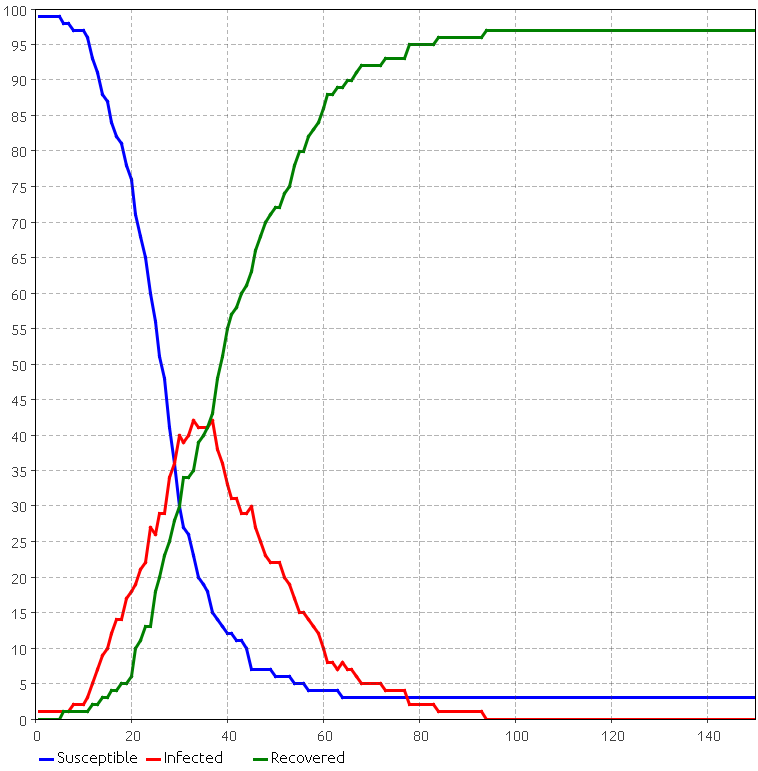
\includegraphics[width=.7\textwidth, angle=0]{./fig/SIR_ABS_ANYLOGIC_100Agents.png}
			\caption{100 Agents}
			\label{fig:pd_seq}
		\end{subfigure}
    	&
		\begin{subfigure}[b]{0.3\textwidth}
			\centering
			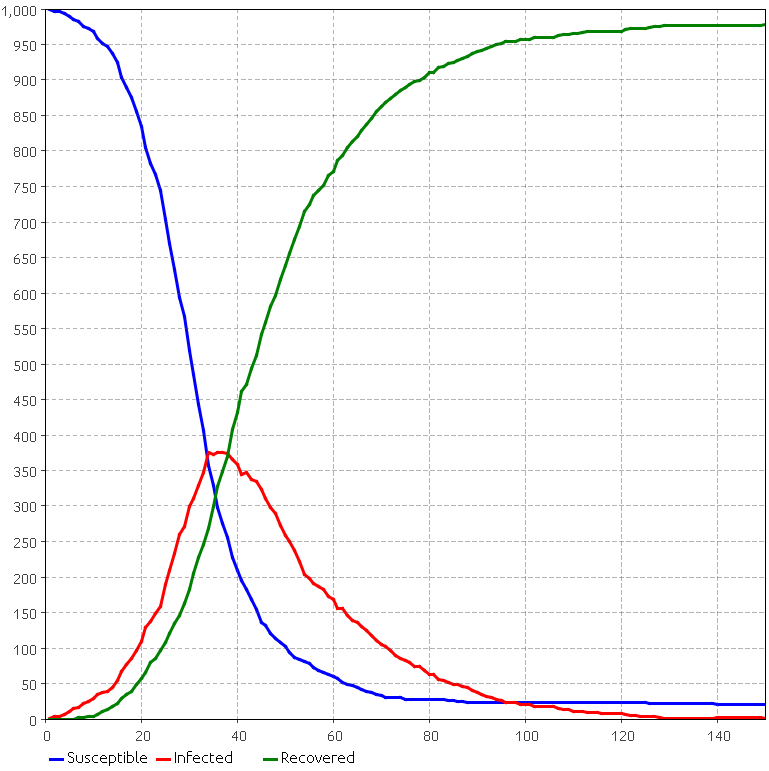
\includegraphics[width=.7\textwidth, angle=0]{./fig/SIR_ABS_ANYLOGIC_1000Agents.png}
			\caption{1000 Agents}
			\label{fig:pd_seq}
		\end{subfigure}
    	&
		\begin{subfigure}[b]{0.3\textwidth}
			\centering
			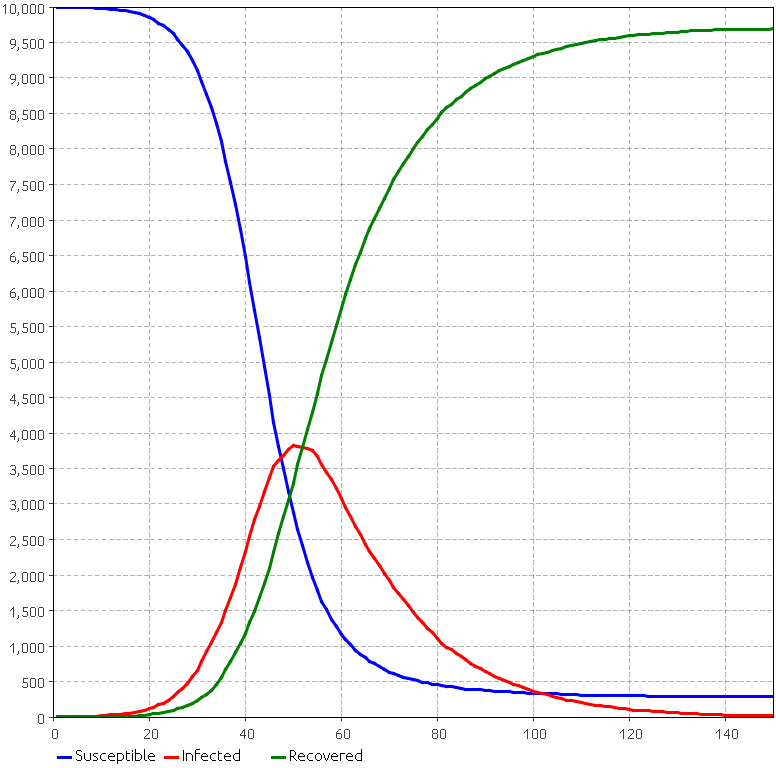
\includegraphics[width=.7\textwidth, angle=0]{./fig/SIR_ABS_ANYLOGIC_10000Agents.png}
			\caption{10,000 Agents}
			\label{fig:hac_seq}
		\end{subfigure}
	\end{tabular}
	
	\caption{\small Approximating the continuous dynamics of the SD simulation using the agent-based approach. Model-parameters are the same ($\beta = 1/5$, $\gamma = 0.05$, $\delta = 15$, 1 initially infected agent) except population size. All Simulations run for 150 time-steps. Dynamics generated with AnyLogic Personal Learning Edition 8.1.0.} 
	\label{fig:sir_abs_anylogic_agents}
\end{center}
\end{figure*}

As previously mentioned the agent-based approach is a rather discrete one which means that with increasing number of agents, the discrete dynamics aproximate the continuous dynamics of the SD simulation. Still the dynamics of 10,000 Agents do not match the dynamics of the SD simulation to a satisfactory level as the Susceptibles in SD fall off earlier and the peak is reached a bit eralier. This is because as opposed to the SD simulation the agent-based approach is inherently a stochastic one as we continuously draw from random-distributions which drive our state-transitions. What we see in Figure \ref{fig:sir_abs_anylogic_agents} is then just a single run where the dynamics would result in slightly different shapes when run with a different random-number generator seed. The agent-based approach thus generates a distribution of dynamics over which ones needs to average to arrive at the correct solution. This can be done using replications in which the simulation is run with the exact same parameteres multiple times but each with a different random-number generator see. The resulting dynamics are then averaged and the result is then regarded as the correct dynamics. We have done this as can be seen in Figure \ref{fig:sir_abs_anylogic_agents_repls}, using 1000 replications, which now completely matches the SD dynamics. \footnote{Note that in the replications we are using 10 initially infected agents to ensure that no simulation run will terminate too early (meaning that the disease gets exstinct after a few time steps) which would offset the dynamics completely. This happens due to "unlucky" random distributions which can be repaired by introducing more initially infected agents which increases the probability of spreading the disease in the very early stage of the simulation drastically. We found that when using 10 initially infected agents in a population of 10,000 (which amounts to (0.1\%)) is enough to never result in an early terminating simulation.}

\begin{figure}
	\centering
	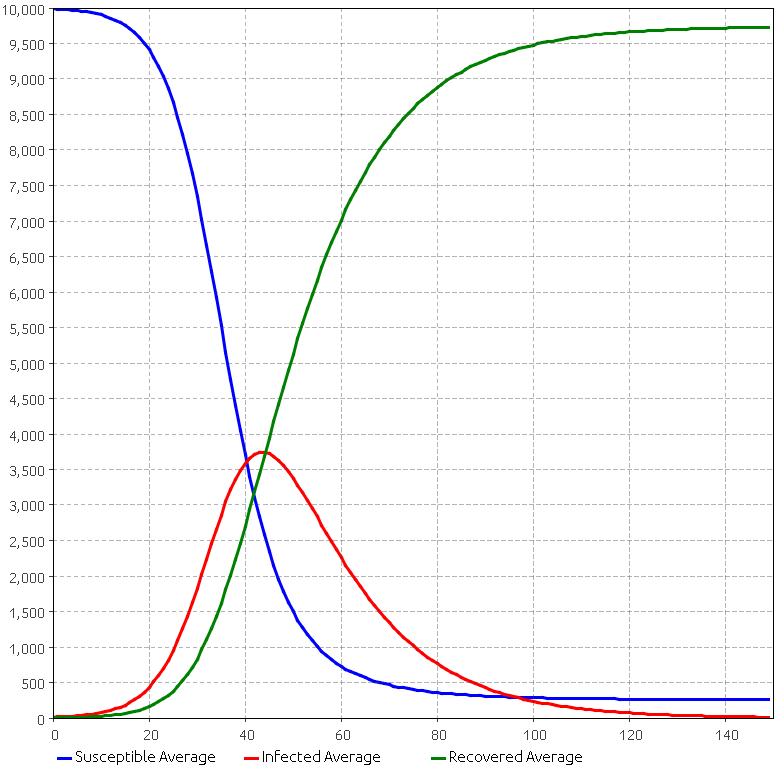
\includegraphics[width=.4\textwidth, angle=0]{./fig/SIR_ABS_ANYLOGIC_10000Agents_10Init_1000Repls.png}
	\caption{Dynamics of the SIR compartment model using the agent-based approach with same parameters as in SD ($\beta = 1/5$, $\gamma = 0.05$, $\delta = 15$) but with a population of 10,000 where 10 are initially infected and the dynamics averaged over 1000 replications. Dynamics generated with AnyLogic Personal Learning Edition 8.1.0.}
	\label{fig:sir_abs_anylogic_agents_repls}
\end{figure}

TODO: cite papers which discuss how to approximate a SD model by ABS: Borshchev, Filippov (2004), Macal (2010)
- Macal (2010) - To Agent-Based Simulation From System Dynamics 
	-> i am bit unhappy with this paper as it does not give concrete parameters for the SD model so it is impossible to replicate. 

- Borshchev, Filippov (2004) - From System Dynamics and Discrete Event to Practical Agent Based Modeling: Reasons, Techniques, Tools
	-> its VERY IMPORTANT point is that we need to draw the illness-duration from an exponential-distribution because the illness-duration is proportional to the size of the infected. note: this is wrongly expressed, need to find the correct formulation